% \title{Desktop Calendar (fits 3.5" floppy disk jewel case)}

%%% The calendars are printed 2-up to fit CD jewel cases,
%%% or 4-up to fit 3" floppy disk jewel cases. OR, now a
%%% full-blown "giant" version that prints full-page!
%%%
%%% Localisation possible with languages supported by
%%% babel/translator/datetime2.
%%% Tested with british, spanish, french, ngerman,
%%% italian, portuges, polish, croatian, greek
%%%
%%% (Use lualatex for french. If using pdflatex for greek,
%%% Remember to load LGR,T1 for fontenc.)
\documentclass[9pt,british,small]{cdcalendar}
%%% Use the sundayweek option for weeks to start on Sundays.
% \documentclass[9pt,british,small,sundayweek]{cdcalendar}

%% If using pdfLaTeX %%%%%%%%%%%%%%%%%%%%%%%%%%
\usepackage[utf8]{inputenc}
\usepackage[T1]{fontenc}

% Using Gentium and Open Sans
\usepackage[utopia]{mathdesign}
\usepackage{ebgaramond}
\usepackage[defaultsans,osfigures,scale=0.94]{opensans}
%% End pdfLaTeX-related font settings %%%%%%%%


% %% Compile with luaLaTeX if using fontspec %%%%%%
% \usepackage{fontspec}
% \setmainfont{Gentium}
% \setsansfont[BoldItalicFont=Fira Sans Italic,BoldFont=Fira Sans]{Fira Sans Light}
% %% End luaLaTeX-related font settings %%%%%%%%%%%

\usepackage{graphicx}
\usepackage{wallpaper}
\usepackage{fontawesome}
\graphicspath{{img/}}
\usepackage[fleqn]{amsmath}

\tikzset{blue icon/.style={text=SkyBlue,font=\Large}}
\tikzset{pink icon/.style={text=Pink,font=\large}}
\tikzset{holiday/.style={rectangle,fill=orange!70}}

\begin{document}

%%%%%%
% Cover
%%%%%%
\coverBgColor{RoyalBlue!40!black}
\coverImage[\color{gray!50}David R.~Goodsell, RCSB PDB, 2005. `Molecule of the Month 2005 August: Neurotrophins: Receptors for nerve growth factor'. \mbox{CC-BY-4.0.} \url{https://doi.org/10.2210/rcsb_pdb/mom_2005_8}]
{68-Neurotrophins-receptors}
\coverTitle[font=\fontsize{20pt}{22pt}\sffamily\bfseries,text=white,text width=\linewidth,align=flush right]{2017 Calendar}

\makeCover

%%%% Remove this page if you don't need it --
%%%% just to show the actual output
{\centering
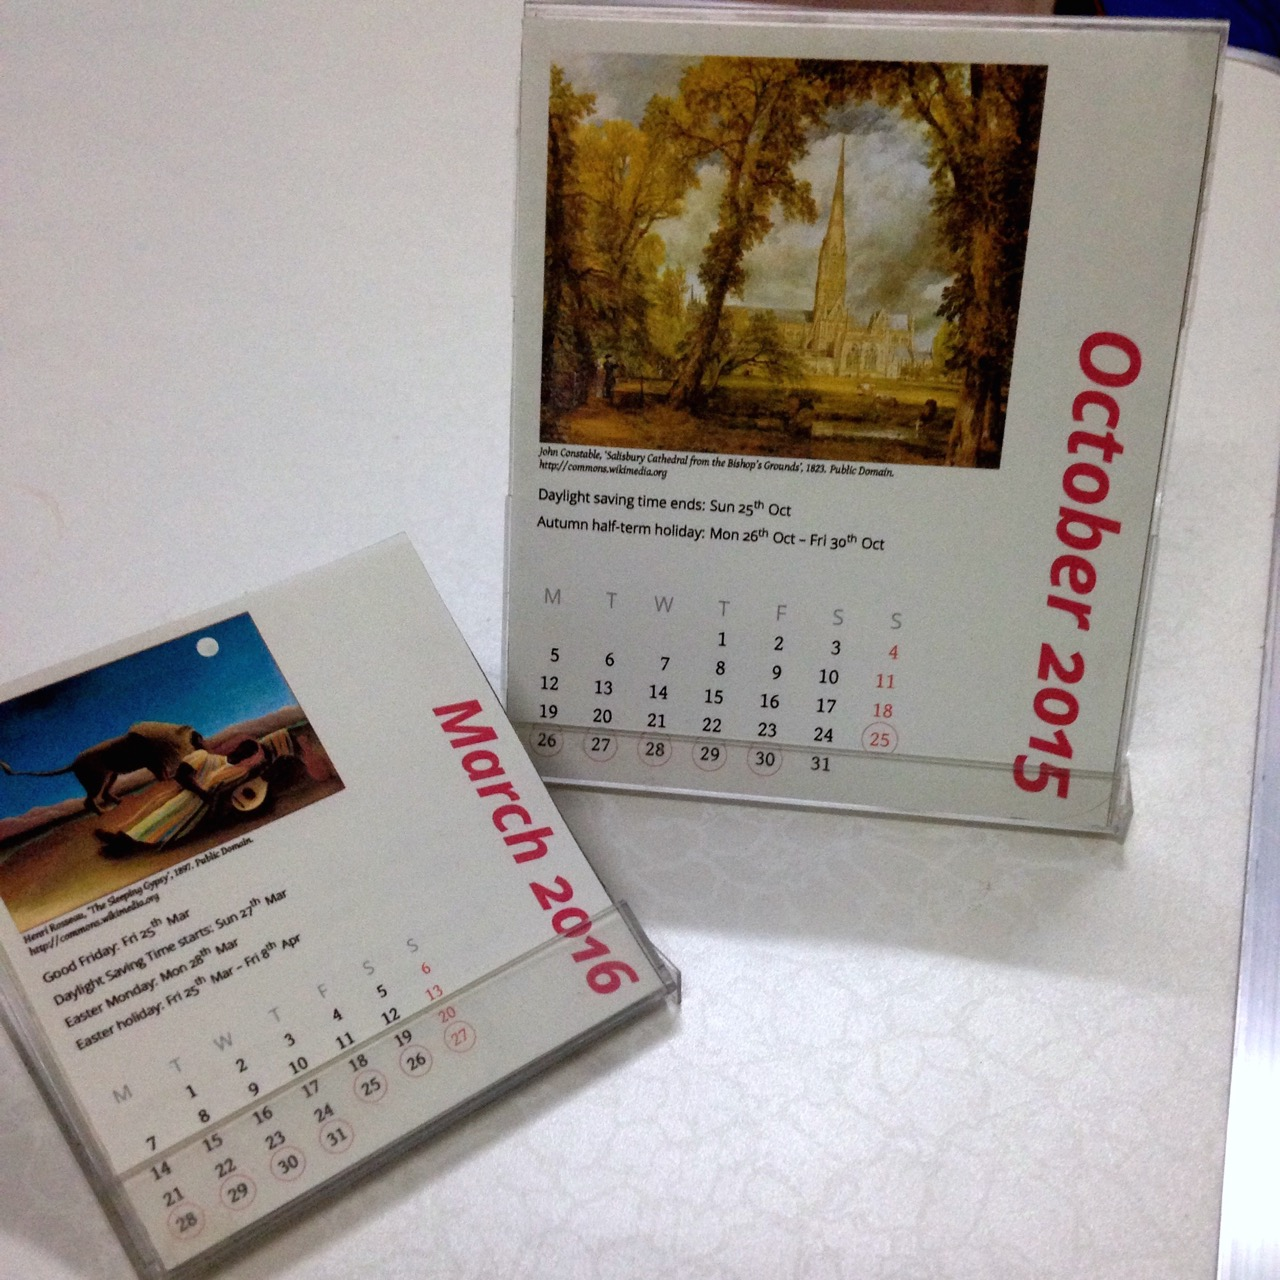
\includegraphics[width=.9\textwidth]{actual}
\par}

Here are the actual printed calendars. The smaller calendar (9\,cm $\times$ 9.5\,cm) fits floppy disk jewel cases; while the bigger one (11.7\,cm $\times$ 13.65\,cm) fits CD jewel cases.

\clearpage
%%%%

%%%%%%
% Some settings for the monthly calendars
%%%%%%
\dayHeadingStyle{font=\sffamily\color{gray!90}}
\sundayColor{red!80!black}
\monthTitleStyle{font={\fontsize{34pt}{36pt}\bfseries\sffamily\itshape\selectfont}, red!50!RedViolet}
\eventStyle{\scriptsize\sffamily}

% Remove this line if you feel the background pattern is too annoying
\TileWallPaper{.5\paperwidth}{.5\paperheight}{ricepaper_v3}

% You may find the gap between illustrations and events too wide
% Use this length to lessen it
\setlength{\lessIllusSkip}{1em}


%%%%%%
% January 2017
%%%%%%
\illustration
[`Detail of a power 20 mandelbulb made using Visions of Chaos'. By Soler97—Own work, Public Domain. \url{http://bit.ly/2hcn1gM}]
{5.5cm}{1125px-Mandelbulb140a}

\begin{monthCalendar}{2017}{01}

%%% events must be given AFTER \begin{monthCalendar}
%%% Currently you must give events on the same page
%%% as the monthly calendar.

%% This is an one-day event
\event[mark style=holiday]{2017-01-01}{}{New Year's Day}
%% This is a 5-day event
\event[mark style=blue icon,marker=\faBriefcase]{2017-01-30}{5}{ACME Conference}
%% you could also write \event{2017-01-06}{2017-02-03}{ACME Conference}

\end{monthCalendar}

\clearpage
\setlength{\lessIllusSkip}{1ex}

%%%%%%
% Feb 2017
%%%%%%

% Or you can put any stuff, really, with a caption if you want:
\setlength{\mathindent}{0pt}
\otherstuff[Legrange's Equation, one of the `greatest mathematical equations'. \url{http://www.livescience.com/26680-greatest-mathematical-equations.html}]
{5.5cm}{\Huge\[%
  \frac{d}{dt}\left(\frac{\partial \textcolor{red}{L}}{\partial \dot{q}_i}\right) = \frac{\partial \textcolor{red}{L}}{\partial q_i}
\]}

\begin{monthCalendar}{2017}{02}

%% Repeat the event if it spans two months
\event[mark style=blue icon,marker=\faBriefcase]{2017-01-30}{5}{ACME Conference}
\event[mark style=pink icon,marker=\faBirthdayCake]{2017-02-07}{}{Someone's birthday}
\event{2017-02-24}{}{Grant proposal deadline!!}

\end{monthCalendar}

\end{document}
